\begin{enumerate}
    \item
    Vào năm 1849, Hippolyte Fizeau, một nhà Vật lý học người Pháp, đã có một thí nghiệm rất tinh tế để xác định tương đối chính xác giá trị của vận tốc ánh sáng: \\

    Thí nghiệm bao gồm các loại vật dụng: Một \textit{nguồn sáng} có khả năng phát ra một tia sáng, một \textit{bánh răng} có $n$ răng (cho rằng kích thước răng rất nhỏ so với bán kính bánh răng, và các răng cách nhau một đoạn đúng bằng chiều rộng của nó) và có thể quay $f$ vòng trong 1 giây ($f$ tùy chỉnh), một chiếc \textit{gương bán mạ phẳng} (gọi là $G_1$), là gương có khả năng cho ánh sáng đi qua ở một bên và phản xạ tại bên khác, một chiếc \textit{gương phẳng} (gọi là $G_2$) có khả năng phản xạ hoàn toàn. \\

    Thiết lập mô hình thí nghiệm như hình $\ref{fig:01}$, bánh răng cách $G_2$ đoạn $L$, bánh răng cách $G_1$ đoạn $l << L$, mắt cũng cách $G_1$ một đoạn rất nhỏ so với L. Khi bắt đầu xoay bánh răng (thay đổi $f$ từ $0$ lên các giá trị dương), hãy \textbf{thiết lập công thức tính vận tốc ánh sáng} theo $L, n, f$. \\
     
\begin{figure}[!h]
    \centering
    \scalebox{0.9}{
    \begin{tikzpicture}[x=0.75pt,y=0.75pt,yscale=-1,xscale=1]
        %uncomment if require: \path (0,300); %set diagram left start at 0, and has height of 300
        
        %Straight Lines [id:da946853565146766] 
        \draw    (148,74) -- (91,150) ;
        %Straight Lines [id:da26326151786137775] 
        \draw    (141,69) -- (84,145) ;
        %Straight Lines [id:da553727655090636] 
        \draw    (91,150) -- (84,145) ;
        %Straight Lines [id:da14578174611522954] 
        \draw    (148,74) -- (141,69) ;
        
        %Straight Lines [id:da573517396051114] 
        \draw [color={rgb, 255:red, 245; green, 166; blue, 35 }  ,draw opacity=1 ][fill={rgb, 255:red, 248; green, 231; blue, 28 }  ,fill opacity=1 ][line width=1.5]    (47,106.5) -- (523,107) ;
        %Straight Lines [id:da8267520901275645] 
        \draw    (522,63.5) -- (522,146.5) ;
        %Straight Lines [id:da4784100652279808] 
        \draw    (531,63.5) -- (531,146.5) ;
        %Straight Lines [id:da2635146280135121] 
        \draw    (531,63.5) -- (522,63.5) ;
        %Straight Lines [id:da05683460435840115] 
        \draw    (531,146.5) -- (522,146.5) ;
        
        %Shape: Rectangle [id:dp20029360038677502] 
        \draw  [color={rgb, 255:red, 228; green, 224; blue, 224 }  ,draw opacity=1 ][fill={rgb, 255:red, 235; green, 230; blue, 230 }  ,fill opacity=1 ] (212,105) -- (221,105) -- (221,113) -- (212,113) -- cycle ;
        %Shape: Rectangle [id:dp7503662347630085] 
        \draw  [color={rgb, 255:red, 80; green, 77; blue, 77 }  ,draw opacity=1 ][fill={rgb, 255:red, 80; green, 78; blue, 78 }  ,fill opacity=1 ] (212,113) -- (221,113) -- (221,122) -- (212,122) -- cycle ;
        %Shape: Rectangle [id:dp8509213219893421] 
        \draw  [color={rgb, 255:red, 228; green, 224; blue, 224 }  ,draw opacity=1 ][fill={rgb, 255:red, 230; green, 230; blue, 230 }  ,fill opacity=1 ] (212,122) -- (221,122) -- (221,134) -- (212,134) -- cycle ;
        %Shape: Rectangle [id:dp2793882527666036] 
        \draw  [color={rgb, 255:red, 80; green, 77; blue, 77 }  ,draw opacity=1 ][fill={rgb, 255:red, 80; green, 78; blue, 78 }  ,fill opacity=1 ] (212,134) -- (221,134) -- (221,145) -- (212,145) -- cycle ;
        %Shape: Rectangle [id:dp8004959651182222] 
        \draw  [color={rgb, 255:red, 228; green, 224; blue, 224 }  ,draw opacity=1 ][fill={rgb, 255:red, 230; green, 230; blue, 230 }  ,fill opacity=1 ] (212,145) -- (221,145) -- (221,157) -- (212,157) -- cycle ;
        %Shape: Rectangle [id:dp16041634663314164] 
        \draw  [color={rgb, 255:red, 80; green, 77; blue, 77 }  ,draw opacity=1 ][fill={rgb, 255:red, 80; green, 78; blue, 78 }  ,fill opacity=1 ] (212,157) -- (221,157) -- (221,171) -- (212,171) -- cycle ;
        %Shape: Rectangle [id:dp033294367773851086] 
        \draw  [color={rgb, 255:red, 228; green, 224; blue, 224 }  ,draw opacity=1 ][fill={rgb, 255:red, 230; green, 230; blue, 230 }  ,fill opacity=1 ] (212,171) -- (221,171) -- (221,181) -- (212,181) -- cycle ;
        %Shape: Rectangle [id:dp08169770692391176] 
        \draw  [color={rgb, 255:red, 80; green, 77; blue, 77 }  ,draw opacity=1 ][fill={rgb, 255:red, 80; green, 78; blue, 78 }  ,fill opacity=1 ] (212,181) -- (221,181) -- (221,192) -- (212,192) -- cycle ;
        %Shape: Rectangle [id:dp3191220518317601] 
        \draw  [color={rgb, 255:red, 228; green, 224; blue, 224 }  ,draw opacity=1 ][fill={rgb, 255:red, 230; green, 230; blue, 230 }  ,fill opacity=1 ] (212,192) -- (221,192) -- (221,202) -- (212,202) -- cycle ;
        %Shape: Rectangle [id:dp9741379806418511] 
        \draw  [color={rgb, 255:red, 80; green, 77; blue, 77 }  ,draw opacity=1 ][fill={rgb, 255:red, 80; green, 78; blue, 78 }  ,fill opacity=1 ] (212,202) -- (221,202) -- (221,208) -- (212,208) -- cycle ;
        %Straight Lines [id:da4523430594635638] 
        \draw [color={rgb, 255:red, 245; green, 166; blue, 35 }  ,draw opacity=1 ][fill={rgb, 255:red, 248; green, 231; blue, 28 }  ,fill opacity=1 ][line width=1.5]    (116,118) -- (522,118) ;
        %Straight Lines [id:da49541126563251425] 
        \draw [color={rgb, 255:red, 245; green, 166; blue, 35 }  ,draw opacity=1 ][line width=1.5]    (116,118) -- (116,126) -- (116,205) ;
        %Straight Lines [id:da9841255686505828] 
        \draw  [dash pattern={on 4.5pt off 4.5pt}]  (220,81) -- (519,81) ;
        \draw [shift={(521,81)}, rotate = 180] [color={rgb, 255:red, 0; green, 0; blue, 0 }  ][line width=0.75]    (10.93,-3.29) .. controls (6.95,-1.4) and (3.31,-0.3) .. (0,0) .. controls (3.31,0.3) and (6.95,1.4) .. (10.93,3.29)   ;
        %Straight Lines [id:da6180566944303607] 
        \draw  [dash pattern={on 4.5pt off 4.5pt}]  (238,81) -- (215,81) ;
        \draw [shift={(213,81)}, rotate = 360] [color={rgb, 255:red, 0; green, 0; blue, 0 }  ][line width=0.75]    (10.93,-3.29) .. controls (6.95,-1.4) and (3.31,-0.3) .. (0,0) .. controls (3.31,0.3) and (6.95,1.4) .. (10.93,3.29)   ;
        
        %Curve Lines [id:da23708665211558855] 
        \draw    (231,143) .. controls (232,128) and (239,129) .. (240,145) ;
        %Straight Lines [id:da2301653905208756] 
        \draw    (231,143) -- (231,159) ;
        %Straight Lines [id:da5360553932392074] 
        \draw    (240,145) -- (240,178) ;
        \draw [shift={(240,180)}, rotate = 270] [color={rgb, 255:red, 0; green, 0; blue, 0 }  ][line width=0.75]    (10.93,-3.29) .. controls (6.95,-1.4) and (3.31,-0.3) .. (0,0) .. controls (3.31,0.3) and (6.95,1.4) .. (10.93,3.29)   ;
        
        %Curve Lines [id:da0685739060837165] 
        \draw [line width=1.5]    (97,233.25) .. controls (109.58,222.25) and (123.42,222.25) .. (136,233.25) ;
        %Curve Lines [id:da6587443364692769] 
        \draw [line width=1.5]    (97,233.25) .. controls (105.81,244.26) and (128.45,242.88) .. (136,233.25) ;
        %Shape: Ellipse [id:dp01919433370631629] 
        \draw  [fill={rgb, 255:red, 0; green, 0; blue, 0 }  ,fill opacity=1 ] (112.1,230.5) .. controls (112.1,227.46) and (114.35,225) .. (117.13,225) .. controls (119.91,225) and (122.16,227.46) .. (122.16,230.5) .. controls (122.16,233.54) and (119.91,236) .. (117.13,236) .. controls (114.35,236) and (112.1,233.54) .. (112.1,230.5) -- cycle ;
        %Shape: Ellipse [id:dp06309375000304929] 
        \draw  [color={rgb, 255:red, 255; green, 255; blue, 255 }  ,draw opacity=1 ][fill={rgb, 255:red, 255; green, 255; blue, 255 }  ,fill opacity=1 ] (115.09,227.89) .. controls (115.14,228.85) and (114.44,229.67) .. (113.53,229.74) .. controls (112.61,229.8) and (111.82,229.08) .. (111.77,228.12) .. controls (111.71,227.17) and (112.41,226.34) .. (113.33,226.28) .. controls (114.24,226.21) and (115.03,226.94) .. (115.09,227.89) -- cycle ;
        
        %Straight Lines [id:da7199316754442766] 
        \draw [line width=1.5]    (92,223) -- (99,226) ;
        %Straight Lines [id:da23147918809452417] 
        \draw [line width=1.5]    (103,215) -- (108,222) ;
        %Straight Lines [id:da02630812195123089] 
        \draw [line width=1.5]    (116.13,220) -- (116,211) ;
        %Straight Lines [id:da5773398495267441] 
        \draw [line width=1.5]    (130,215) -- (124,221) ;
        %Straight Lines [id:da7344993546008041] 
        \draw [line width=1.5]    (133,225) -- (141,222) ;
        
        \draw  [color={rgb, 255:red, 245; green, 166; blue, 35 }  ,draw opacity=1 ] (311,102) -- (321,107) -- (311,112) ;
        \draw  [color={rgb, 255:red, 245; green, 166; blue, 35 }  ,draw opacity=1 ] (386.91,123.09) -- (377,117.91) -- (387.09,113.09) ;
        \draw  [color={rgb, 255:red, 245; green, 166; blue, 35 }  ,draw opacity=1 ] (120.93,150.93) -- (116.07,161) -- (110.93,151.07) ;
        %Image [id:dp5013590793864575] 
        \draw (338,238) node  {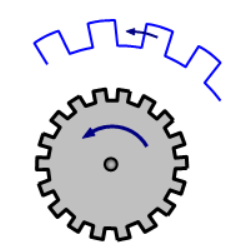
\includegraphics[width=63pt,height=63pt]{Problem_5/Wheel.png}};
        %Straight Lines [id:da6111860060741341] 
        \draw    (299,242) -- (233.78,208.91) ;
        \draw [shift={(232,208)}, rotate = 26.91] [color={rgb, 255:red, 0; green, 0; blue, 0 }  ][line width=0.75]    (10.93,-3.29) .. controls (6.95,-1.4) and (3.31,-0.3) .. (0,0) .. controls (3.31,0.3) and (6.95,1.4) .. (10.93,3.29)   ;
        
        % Text Node
        \draw (140,42.4) node [anchor=north west][inner sep=0.75pt]    {$G_{1}$};
        % Text Node
        \draw (515,39.4) node [anchor=north west][inner sep=0.75pt]    {$G_{2}$};
        % Text Node
        \draw (360,57.4) node [anchor=north west][inner sep=0.75pt]    {$L$};
        % Text Node
        \draw (245,141.4) node [anchor=north west][inner sep=0.75pt]    {$f$};
        
        
    \end{tikzpicture}
    }
    
    \caption{Mô hình thực nghiệm của Fizeau}
    \label{fig:01}
\end{figure}

    \item Thay $L = \SI{8630}{m}$, $n = 720$ bánh răng, và khi hiện tượng cần tìm xảy ra, $f = 12.6$ vòng/s để tính vận tốc ánh sáng dựa trên thí nghiệm này. Tính phần trăm chênh lệch giữa giá trị vừa tính được và giá trị chính xác hiện nay ($c = \SI{299 792 458}{m/s}$).

    \item
    Sau khi có được giá trị của vận tốc ánh sáng, Léon Foucault, cộng sự của Fizeau, đã phát triển thêm cho thí nghiệm này vào năm 1862 bằng việc sử dụng một chiếc gương quay thay cho bánh răng: \\

    Thí nghiệm bao gồm các vật dụng: Một chiếc \textit{gương bán mạ} (gọi là $G_3$) được gắn cố định, một chiếc \textit{gương phẳng} (gọi là $G_4$) có khả năng phản xạ toàn phần, được \textit{gắn trên một motor} có khả năng xoay qua một trục cố định với và có thể quay $f$ vòng trong 1 giây ($f$ tùy chỉnh), một chiếc \textit{gương phẳng khác} (gọi là $G_5$) được gắn cố định, một tấm kính mờ để đón ánh sáng, một \textit{nguồn sáng} có khả năng phát ra một tia sáng (trên thực tế, còn có thêm một \textit{thấu kính hội tụ} để tránh trường hợp các tia sáng loe ra khi phản xạ tại $G_5$, nhưng trong thí nghiệm này, ta giả sử \textbf{mọi điều kiện về ánh sáng đủ hoàn hảo để không bị loe ra trong quá trình truyền}). \\

    Thiết lập mô hình thí nghiệm như hình $\ref{fig:02}$. Gương $G_3$ cách gương $G_4$ đoạn R, gương $G_4$ cách gương $G_5$ đoạn D. Nếu gương $G_4$ không xoay thì đường truyền ánh sáng va vào tấm kính mờ $E$ sẽ là đường nét đứt. Khi bắt đầu xoay gương $G_4$ với tần số $f$ (vòng/s) thì điểm mà tia sáng chiếu tới tấm $E$ sẽ cách điểm ban đầu đoạn $\Delta x$. Hãy \textbf{thiết lập công thức tính vận tốc ánh sáng} theo $D, R, x, f$.

\begin{figure}[!h]
    \centering
    \scalebox{0.9}{
    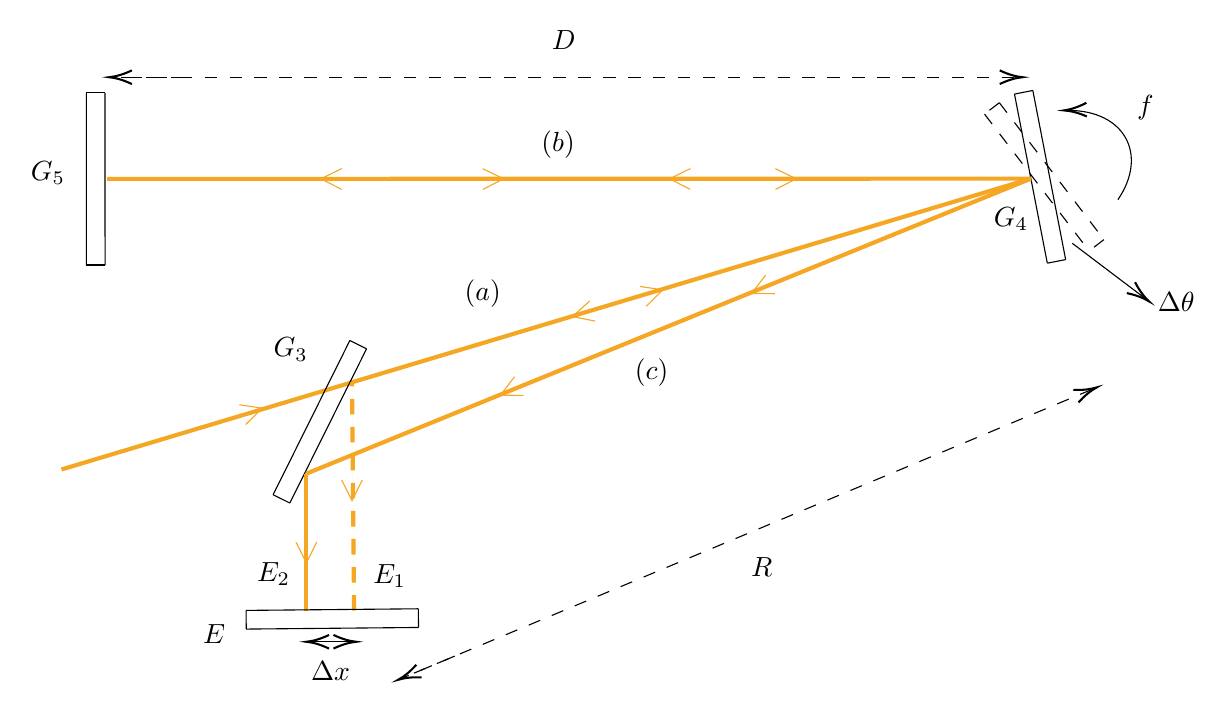
\begin{tikzpicture}[x=0.75pt,y=0.75pt,yscale=-1,xscale=1]
        %uncomment if require: \path (0,376); %set diagram left start at 0, and has height of 376
        
        %Straight Lines [id:da45181753303075034] 
        \draw [color={rgb, 255:red, 245; green, 166; blue, 35 }  ,draw opacity=1 ][fill={rgb, 255:red, 248; green, 231; blue, 28 }  ,fill opacity=1 ][line width=1.5]    (62,223) -- (529.08,82.86) ;
        %Straight Lines [id:da37095602442747344] 
        \draw    (521.17,42.12) -- (536.99,123.6) ;
        %Straight Lines [id:da9613423099187735] 
        \draw    (530.01,40.4) -- (545.83,121.88) ;
        %Straight Lines [id:da5222176524623936] 
        \draw    (530.01,40.4) -- (521.17,42.12) ;
        %Straight Lines [id:da3602031691061027] 
        \draw    (545.83,121.88) -- (536.99,123.6) ;
        
        %Straight Lines [id:da31811781190469146] 
        \draw [color={rgb, 255:red, 245; green, 166; blue, 35 }  ,draw opacity=1 ][fill={rgb, 255:red, 245; green, 166; blue, 35 }  ,fill opacity=1 ][line width=1.5]    (84,83) -- (529.08,82.86) ;
        %Straight Lines [id:da007553168479752959] 
        \draw    (73.98,41.5) -- (74.02,124.5) ;
        %Straight Lines [id:da41646702673961] 
        \draw    (82.98,41.5) -- (83.02,124.5) ;
        %Straight Lines [id:da831986993347021] 
        \draw    (82.98,41.5) -- (73.98,41.5) ;
        %Straight Lines [id:da1725078310294783] 
        \draw    (83.02,124.5) -- (74.02,124.5) ;
        
        \draw  [color={rgb, 255:red, 245; green, 166; blue, 35 }  ,draw opacity=1 ] (364.98,88.02) -- (355,82.98) -- (365.02,78.02) ;
        \draw  [color={rgb, 255:red, 245; green, 166; blue, 35 }  ,draw opacity=1 ] (196.98,88.02) -- (187,82.98) -- (197.02,78.02) ;
        \draw  [color={rgb, 255:red, 245; green, 166; blue, 35 }  ,draw opacity=1 ] (264.95,78.06) -- (275,82.95) -- (265.06,88.05) ;
        \draw  [color={rgb, 255:red, 245; green, 166; blue, 35 }  ,draw opacity=1 ] (405.95,78.06) -- (416,82.95) -- (406.06,88.05) ;
        \draw  [color={rgb, 255:red, 245; green, 166; blue, 35 }  ,draw opacity=1 ] (147.69,191.81) -- (158.75,193.44) -- (150.81,201.31) ;
        \draw  [color={rgb, 255:red, 245; green, 166; blue, 35 }  ,draw opacity=1 ] (340.69,134.81) -- (351.75,136.44) -- (343.81,144.31) ;
        %Straight Lines [id:da6709803355219819] 
        \draw  [dash pattern={on 4.5pt off 4.5pt}]  (506.73,51.75) -- (557.12,117.71) ;
        %Straight Lines [id:da26309567784103494] 
        \draw  [dash pattern={on 4.5pt off 4.5pt}]  (513.88,46.29) -- (564.27,112.25) ;
        %Straight Lines [id:da19545875237692845] 
        \draw  [dash pattern={on 4.5pt off 4.5pt}]  (513.88,46.29) -- (506.73,51.75) ;
        
        %Straight Lines [id:da4908738819121423] 
        \draw  [dash pattern={on 4.5pt off 4.5pt}]  (564.27,112.25) -- (557.12,117.71) ;
        
        %Straight Lines [id:da8989986144809015] 
        \draw    (200.96,160.84) -- (163.99,235.15) ;
        %Straight Lines [id:da9518792064296806] 
        \draw    (209.01,164.85) -- (172.04,239.16) ;
        %Straight Lines [id:da7757940083119736] 
        \draw    (209.01,164.85) -- (200.96,160.84) ;
        %Straight Lines [id:da012215162664961143] 
        \draw    (172.04,239.16) -- (163.99,235.15) ;
        
        %Straight Lines [id:da5855486248930339] 
        \draw [color={rgb, 255:red, 245; green, 166; blue, 35 }  ,draw opacity=1 ][fill={rgb, 255:red, 248; green, 231; blue, 28 }  ,fill opacity=1 ][line width=1.5]    (180,225) -- (529.08,82.86) ;
        %Straight Lines [id:da0018983805533445697] 
        \draw [color={rgb, 255:red, 245; green, 166; blue, 35 }  ,draw opacity=1 ][fill={rgb, 255:red, 248; green, 231; blue, 28 }  ,fill opacity=1 ][line width=1.5]  [dash pattern={on 5.63pt off 4.5pt}]  (203,291) -- (202,181) ;
        %Straight Lines [id:da9093747338461293] 
        \draw [color={rgb, 255:red, 245; green, 166; blue, 35 }  ,draw opacity=1 ][fill={rgb, 255:red, 248; green, 231; blue, 28 }  ,fill opacity=1 ][line width=1.5]    (180,291) -- (180,225) ;
        %Straight Lines [id:da12015375747814039] 
        \draw    (233.96,290.11) -- (150.96,290.89) ;
        %Straight Lines [id:da5642208049777369] 
        \draw    (234.04,299.11) -- (151.04,299.89) ;
        %Straight Lines [id:da197599021789286] 
        \draw    (234.04,299.11) -- (233.96,290.11) ;
        %Straight Lines [id:da112866013313629] 
        \draw    (151.04,299.89) -- (150.96,290.89) ;
        
        %Straight Lines [id:da3164840887041933] 
        \draw  [dash pattern={on 4.5pt off 4.5pt}]  (95,34) -- (523,34) ;
        \draw [shift={(525,34)}, rotate = 180] [color={rgb, 255:red, 0; green, 0; blue, 0 }  ][line width=0.75]    (10.93,-3.29) .. controls (6.95,-1.4) and (3.31,-0.3) .. (0,0) .. controls (3.31,0.3) and (6.95,1.4) .. (10.93,3.29)   ;
        %Straight Lines [id:da04320074999405121] 
        \draw  [dash pattern={on 4.5pt off 4.5pt}]  (120.71,34) -- (87,34) ;
        \draw [shift={(85,34)}, rotate = 360] [color={rgb, 255:red, 0; green, 0; blue, 0 }  ][line width=0.75]    (10.93,-3.29) .. controls (6.95,-1.4) and (3.31,-0.3) .. (0,0) .. controls (3.31,0.3) and (6.95,1.4) .. (10.93,3.29)   ;
        
        %Straight Lines [id:da09034280950418583] 
        \draw  [dash pattern={on 4.5pt off 4.5pt}]  (231.8,321.14) -- (559.01,184.2) ;
        \draw [shift={(560.85,183.43)}, rotate = 157.29] [color={rgb, 255:red, 0; green, 0; blue, 0 }  ][line width=0.75]    (10.93,-3.29) .. controls (6.95,-1.4) and (3.31,-0.3) .. (0,0) .. controls (3.31,0.3) and (6.95,1.4) .. (10.93,3.29)   ;
        %Straight Lines [id:da9181861084457834] 
        \draw  [dash pattern={on 4.5pt off 4.5pt}]  (251.48,312.91) -- (225.99,323.58) ;
        \draw [shift={(224.15,324.35)}, rotate = 337.29] [color={rgb, 255:red, 0; green, 0; blue, 0 }  ][line width=0.75]    (10.93,-3.29) .. controls (6.95,-1.4) and (3.31,-0.3) .. (0,0) .. controls (3.31,0.3) and (6.95,1.4) .. (10.93,3.29)   ;
        
        %Straight Lines [id:da5936626087488515] 
        \draw    (180,306) -- (202,306) ;
        \draw [shift={(204,306)}, rotate = 180] [color={rgb, 255:red, 0; green, 0; blue, 0 }  ][line width=0.75]    (10.93,-3.29) .. controls (6.95,-1.4) and (3.31,-0.3) .. (0,0) .. controls (3.31,0.3) and (6.95,1.4) .. (10.93,3.29)   ;
        %Straight Lines [id:da7915781509760136] 
        \draw    (192,306) -- (182,306) ;
        \draw [shift={(180,306)}, rotate = 360] [color={rgb, 255:red, 0; green, 0; blue, 0 }  ][line width=0.75]    (10.93,-3.29) .. controls (6.95,-1.4) and (3.31,-0.3) .. (0,0) .. controls (3.31,0.3) and (6.95,1.4) .. (10.93,3.29)   ;
        %Straight Lines [id:da17868012118393306] 
        \draw    (549,114) -- (584.41,140.79) ;
        \draw [shift={(586,142)}, rotate = 217.12] [color={rgb, 255:red, 0; green, 0; blue, 0 }  ][line width=0.75]    (10.93,-3.29) .. controls (6.95,-1.4) and (3.31,-0.3) .. (0,0) .. controls (3.31,0.3) and (6.95,1.4) .. (10.93,3.29)   ;
        \draw  [color={rgb, 255:red, 245; green, 166; blue, 35 }  ,draw opacity=1 ] (405.68,138.31) -- (394.5,138.19) -- (401.31,129.32) ;
        \draw  [color={rgb, 255:red, 245; green, 166; blue, 35 }  ,draw opacity=1 ] (284.68,187.31) -- (273.5,187.19) -- (280.31,178.32) ;
        \draw  [color={rgb, 255:red, 245; green, 166; blue, 35 }  ,draw opacity=1 ] (319.15,151.5) -- (308.18,149.33) -- (316.5,141.85) ;
        \draw  [color={rgb, 255:red, 245; green, 166; blue, 35 }  ,draw opacity=1 ] (206.99,227.99) -- (202.01,238) -- (196.99,228.01) ;
        \draw  [color={rgb, 255:red, 245; green, 166; blue, 35 }  ,draw opacity=1 ] (184.99,257.99) -- (180.01,268) -- (174.99,258.01) ;
        %Curve Lines [id:da7809444350892587] 
        \draw    (571,93) .. controls (585.7,71.44) and (574.47,49.88) .. (546.72,49.97) ;
        \draw [shift={(545,50)}, rotate = 358.03] [color={rgb, 255:red, 0; green, 0; blue, 0 }  ][line width=0.75]    (10.93,-3.29) .. controls (6.95,-1.4) and (3.31,-0.3) .. (0,0) .. controls (3.31,0.3) and (6.95,1.4) .. (10.93,3.29)   ;
        
        % Text Node
        \draw (297,10.4) node [anchor=north west][inner sep=0.75pt]    {$D$};
        % Text Node
        \draw (393,264.4) node [anchor=north west][inner sep=0.75pt]    {$R$};
        % Text Node
        \draw (181,314.4) node [anchor=north west][inner sep=0.75pt]    {$\Delta x$};
        % Text Node
        \draw (163,158.4) node [anchor=north west][inner sep=0.75pt]    {$G_{3}$};
        % Text Node
        \draw (510,95.4) node [anchor=north west][inner sep=0.75pt]    {$G_{4}$};
        % Text Node
        \draw (46,73.4) node [anchor=north west][inner sep=0.75pt]    {$G_{5}$};
        % Text Node
        \draw (589,136.4) node [anchor=north west][inner sep=0.75pt]    {$\Delta \theta $};
        % Text Node
        \draw (129,296.4) node [anchor=north west][inner sep=0.75pt]    {$E$};
        % Text Node
        \draw (579,41.4) node [anchor=north west][inner sep=0.75pt]    {$f$};
        % Text Node
        \draw (255,130.4) node [anchor=north west][inner sep=0.75pt]    {$( a)$};
        % Text Node
        \draw (292,58.4) node [anchor=north west][inner sep=0.75pt]    {$( b)$};
        % Text Node
        \draw (337,168.4) node [anchor=north west][inner sep=0.75pt]    {$( c)$};
        % Text Node
        \draw (211,267.4) node [anchor=north west][inner sep=0.75pt]    {$E_{1}$};
        % Text Node
        \draw (155,266.4) node [anchor=north west][inner sep=0.75pt]    {$E_{2}$};
        
        
    \end{tikzpicture}
    }
    
    \caption{Mô hình thực nghiệm của Foucault}
    \label{fig:02}
\end{figure}

    \item Dựa vào thí nghiệm này và thay các số liệu cần thiết, ta ra được kết quả $c = \SI{298 000 000}{m/s}$. So sánh kết quả này với gía trị chính xác hiện nay ($c = \SI{299 792 458}{m/s}$) và giá trị của Foucault để xem rằng bản cải tiến của Foucault có hiệu quả hơn không. 

    \textbf{Lưu ý}: Với đơn vị góc Radian mà $360^\circ \equiv 2 \pi \ \si{rad}$, ở góc $x$ nhỏ, ta có thể xấp xỉ $\tan(x) \approx \sin(x) \approx x$.
\end{enumerate}



\begin{flushright}
   \normalcolor(Biên soạn bởi Colevol)
\end{flushright}